\begin{document}
\begin{knitrout}
\definecolor{shadecolor}{rgb}{0.969, 0.969, 0.969}\color{fgcolor}\begin{kframe}
\begin{alltt}
\hlcom{####Problem 9}
\hlstd{r} \hlkwb{=} \hlnum{2.5}
\hlstd{p} \hlkwb{=} \hlnum{5}
\hlcom{###P<=10}
\hlkwd{pgamma}\hlstd{(}\hlkwc{q} \hlstd{=} \hlnum{10}\hlstd{,} \hlkwc{shape} \hlstd{= r,} \hlkwc{scale} \hlstd{= p)}
\end{alltt}
\begin{verbatim}
## [1] 0.450584
\end{verbatim}
\begin{alltt}
\hlkwd{pgamma}\hlstd{(}\hlkwc{q} \hlstd{=} \hlnum{5}\hlstd{,} \hlkwc{shape} \hlstd{= r,} \hlkwc{scale} \hlstd{= p,} \hlkwc{lower.tail} \hlstd{= F)}
\end{alltt}
\begin{verbatim}
## [1] 0.849145
\end{verbatim}
\begin{alltt}
\hlcom{#P(abs(X-8)<3)=P(X<11) & P(X>5) = P(5<X<11)}
\hlkwd{pgamma}\hlstd{(}\hlkwc{q} \hlstd{=} \hlnum{5}\hlstd{,} \hlkwc{shape} \hlstd{= r,} \hlkwc{scale} \hlstd{= p,} \hlkwc{lower.tail} \hlstd{= F)} \hlopt{-} \hlkwd{pgamma}\hlstd{(}\hlkwc{q} \hlstd{=} \hlnum{11}\hlstd{,} \hlkwc{shape} \hlstd{= r,} \hlkwc{scale} \hlstd{= p,} \hlkwc{lower.tail} \hlstd{= F)}
\end{alltt}
\begin{verbatim}
## [1] 0.3557715
\end{verbatim}
\begin{alltt}
\hlstd{i} \hlkwb{=} \hlnum{4}
\hlstd{z} \hlkwb{=} \hlkwd{pgamma}\hlstd{(}\hlkwc{q} \hlstd{= i,} \hlkwc{shape} \hlstd{= r,} \hlkwc{scale} \hlstd{= p)}
\hlkwa{while}\hlstd{(z}\hlopt{<}\hlnum{.1}\hlstd{)\{}
\hlstd{i} \hlkwb{=} \hlstd{i} \hlopt{+} \hlnum{.001}
\hlstd{z} \hlkwb{=} \hlkwd{pgamma}\hlstd{(}\hlkwc{q} \hlstd{= i,} \hlkwc{shape} \hlstd{= r,} \hlkwc{scale} \hlstd{= p)}
\hlstd{\}}
\hlstd{i}
\end{alltt}
\begin{verbatim}
## [1] 4.026
\end{verbatim}
\end{kframe}
\end{knitrout}

\begin{knitrout}
\definecolor{shadecolor}{rgb}{0.969, 0.969, 0.969}\color{fgcolor}\begin{kframe}
\begin{alltt}
\hlcom{####Problem 10}
\hlstd{x} \hlkwb{=} \hlnum{0}\hlopt{:}\hlnum{20}
\hlkwd{plot}\hlstd{(x,} \hlkwd{pbinom}\hlstd{(x,} \hlnum{20}\hlstd{,} \hlkwc{prob} \hlstd{=} \hlnum{1}\hlopt{/}\hlnum{3}\hlstd{),} \hlkwc{type} \hlstd{=} \hlstr{'s'}\hlstd{)}
\hlkwd{lines}\hlstd{(x,} \hlkwd{phyper}\hlstd{(x,} \hlkwc{m} \hlstd{=} \hlnum{40}\hlstd{,} \hlkwc{n} \hlstd{=} \hlnum{80}\hlstd{,} \hlkwc{k} \hlstd{=} \hlnum{20}\hlstd{),} \hlkwc{type} \hlstd{=} \hlstr{'s'}\hlstd{,} \hlkwc{col} \hlstd{=} \hlstr{"red"}\hlstd{)}
\end{alltt}
\end{kframe}
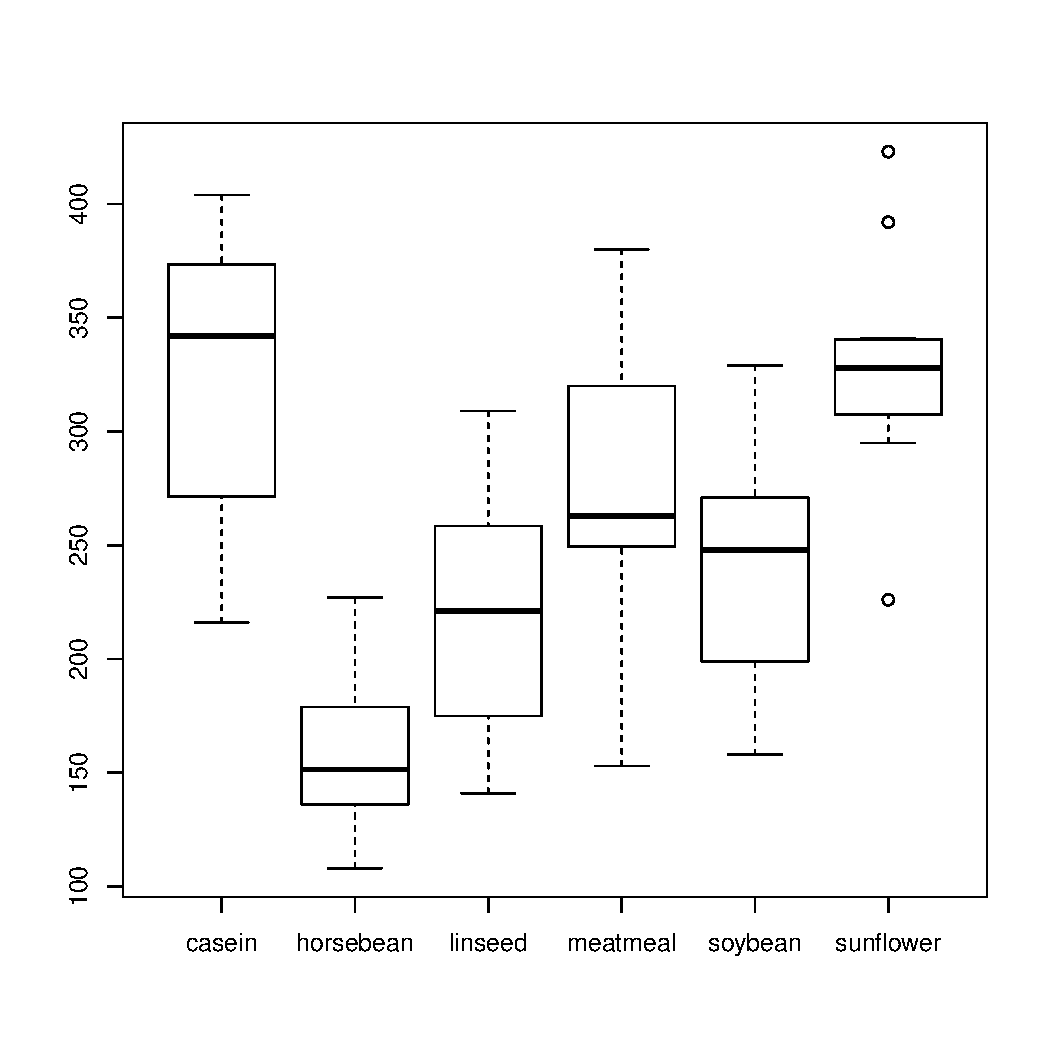
\includegraphics[width=\maxwidth]{figure/unnamed-chunk-2-1} 
\begin{kframe}\begin{alltt}
\hlcom{####Problem 11}
\hlstd{x} \hlkwb{=} \hlnum{0}\hlopt{:}\hlnum{20}
\hlkwd{plot}\hlstd{(x,} \hlkwd{pbinom}\hlstd{(x,} \hlnum{40}\hlstd{,} \hlkwc{prob} \hlstd{=} \hlnum{.3}\hlstd{),} \hlkwc{type} \hlstd{=} \hlstr{'s'}\hlstd{)}
\hlkwd{lines}\hlstd{(x,} \hlkwd{pnorm}\hlstd{(x,} \hlkwc{mean} \hlstd{=} \hlnum{12}\hlstd{,} \hlkwc{sd} \hlstd{=} \hlnum{2.9}\hlstd{),} \hlkwc{type} \hlstd{=} \hlstr{'s'}\hlstd{,} \hlkwc{col} \hlstd{=} \hlstr{"red"}\hlstd{)}
\end{alltt}
\end{kframe}
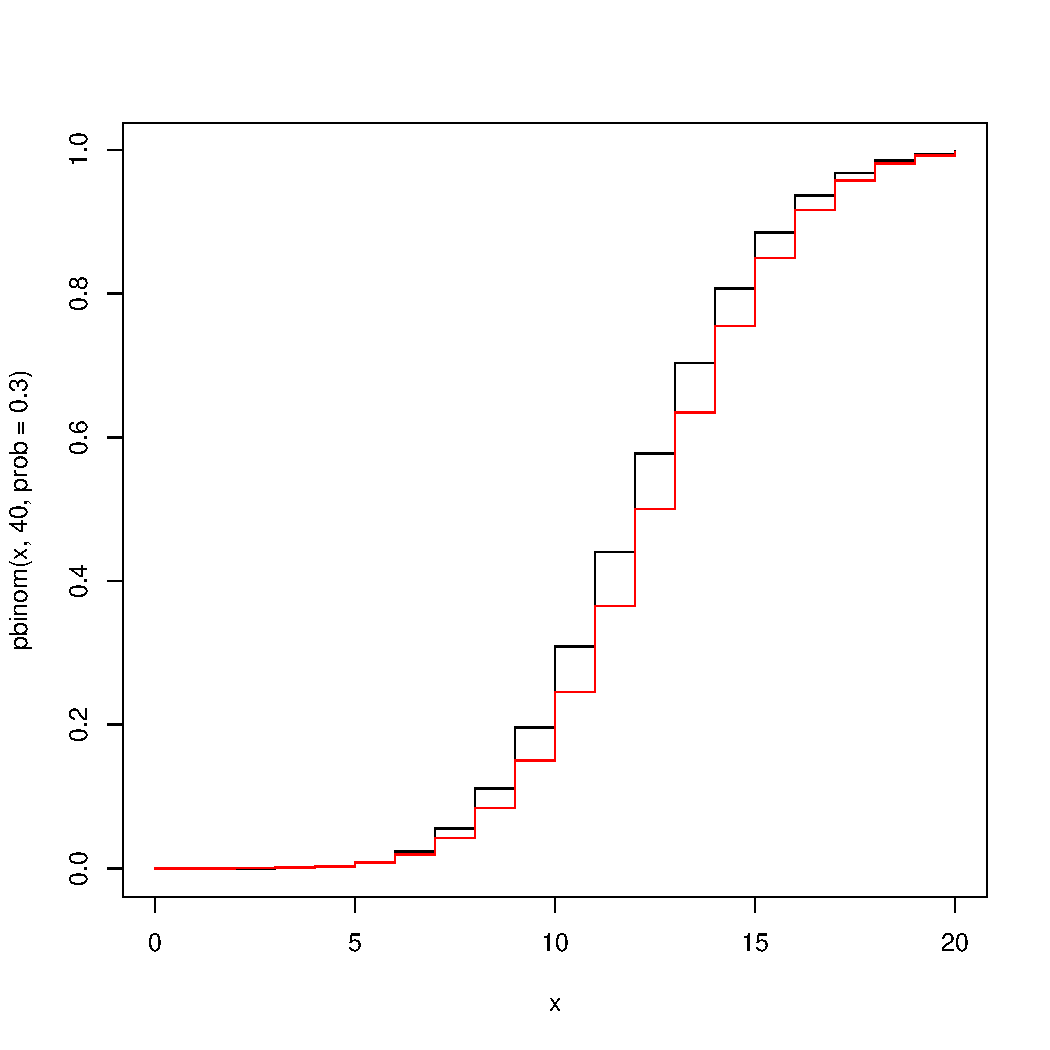
\includegraphics[width=\maxwidth]{figure/unnamed-chunk-2-2} 
\begin{kframe}\begin{alltt}
\hlcom{####Problem 12}
\hlkwd{par}\hlstd{(}\hlkwc{mfrow}\hlstd{=}\hlkwd{c}\hlstd{(}\hlnum{3}\hlstd{,} \hlnum{2}\hlstd{))}
\hlstd{sizes} \hlkwb{=} \hlkwd{c}\hlstd{(}\hlnum{10}\hlstd{,} \hlnum{20}\hlstd{,} \hlnum{40}\hlstd{,} \hlnum{100}\hlstd{,} \hlnum{1000}\hlstd{)}
  \hlkwa{for}\hlstd{(i} \hlkwa{in} \hlstd{sizes)\{}
  \hlkwd{qqnorm}\hlstd{(}\hlkwd{rnorm}\hlstd{(i),} \hlkwc{title} \hlstd{=} \hlkwd{paste}\hlstd{(}\hlkwd{c}\hlstd{(}\hlstr{"sample size"}\hlstd{,} \hlkwd{as.character}\hlstd{(i))))}
  \hlstd{\}}
\end{alltt}


{\ttfamily\noindent\color{warningcolor}{\#\# Warning in plot.window(...): "{}title"{} is not a graphical parameter}}

{\ttfamily\noindent\color{warningcolor}{\#\# Warning in plot.xy(xy, type, ...): "{}title"{} is not a graphical parameter}}

{\ttfamily\noindent\color{warningcolor}{\#\# Warning in axis(side = side, at = at, labels = labels, ...): "{}title"{} is not a graphical parameter}}

{\ttfamily\noindent\color{warningcolor}{\#\# Warning in axis(side = side, at = at, labels = labels, ...): "{}title"{} is not a graphical parameter}}

{\ttfamily\noindent\color{warningcolor}{\#\# Warning in box(...): "{}title"{} is not a graphical parameter}}

{\ttfamily\noindent\color{warningcolor}{\#\# Warning in title(...): "{}title"{} is not a graphical parameter}}

{\ttfamily\noindent\color{warningcolor}{\#\# Warning in plot.window(...): "{}title"{} is not a graphical parameter}}

{\ttfamily\noindent\color{warningcolor}{\#\# Warning in plot.xy(xy, type, ...): "{}title"{} is not a graphical parameter}}

{\ttfamily\noindent\color{warningcolor}{\#\# Warning in axis(side = side, at = at, labels = labels, ...): "{}title"{} is not a graphical parameter}}

{\ttfamily\noindent\color{warningcolor}{\#\# Warning in axis(side = side, at = at, labels = labels, ...): "{}title"{} is not a graphical parameter}}

{\ttfamily\noindent\color{warningcolor}{\#\# Warning in box(...): "{}title"{} is not a graphical parameter}}

{\ttfamily\noindent\color{warningcolor}{\#\# Warning in title(...): "{}title"{} is not a graphical parameter}}

{\ttfamily\noindent\color{warningcolor}{\#\# Warning in plot.window(...): "{}title"{} is not a graphical parameter}}

{\ttfamily\noindent\color{warningcolor}{\#\# Warning in plot.xy(xy, type, ...): "{}title"{} is not a graphical parameter}}

{\ttfamily\noindent\color{warningcolor}{\#\# Warning in axis(side = side, at = at, labels = labels, ...): "{}title"{} is not a graphical parameter}}

{\ttfamily\noindent\color{warningcolor}{\#\# Warning in axis(side = side, at = at, labels = labels, ...): "{}title"{} is not a graphical parameter}}

{\ttfamily\noindent\color{warningcolor}{\#\# Warning in box(...): "{}title"{} is not a graphical parameter}}

{\ttfamily\noindent\color{warningcolor}{\#\# Warning in title(...): "{}title"{} is not a graphical parameter}}

{\ttfamily\noindent\color{warningcolor}{\#\# Warning in plot.window(...): "{}title"{} is not a graphical parameter}}

{\ttfamily\noindent\color{warningcolor}{\#\# Warning in plot.xy(xy, type, ...): "{}title"{} is not a graphical parameter}}

{\ttfamily\noindent\color{warningcolor}{\#\# Warning in axis(side = side, at = at, labels = labels, ...): "{}title"{} is not a graphical parameter}}

{\ttfamily\noindent\color{warningcolor}{\#\# Warning in axis(side = side, at = at, labels = labels, ...): "{}title"{} is not a graphical parameter}}

{\ttfamily\noindent\color{warningcolor}{\#\# Warning in box(...): "{}title"{} is not a graphical parameter}}

{\ttfamily\noindent\color{warningcolor}{\#\# Warning in title(...): "{}title"{} is not a graphical parameter}}

{\ttfamily\noindent\color{warningcolor}{\#\# Warning in plot.window(...): "{}title"{} is not a graphical parameter}}

{\ttfamily\noindent\color{warningcolor}{\#\# Warning in plot.xy(xy, type, ...): "{}title"{} is not a graphical parameter}}

{\ttfamily\noindent\color{warningcolor}{\#\# Warning in axis(side = side, at = at, labels = labels, ...): "{}title"{} is not a graphical parameter}}

{\ttfamily\noindent\color{warningcolor}{\#\# Warning in axis(side = side, at = at, labels = labels, ...): "{}title"{} is not a graphical parameter}}

{\ttfamily\noindent\color{warningcolor}{\#\# Warning in box(...): "{}title"{} is not a graphical parameter}}

{\ttfamily\noindent\color{warningcolor}{\#\# Warning in title(...): "{}title"{} is not a graphical parameter}}\end{kframe}
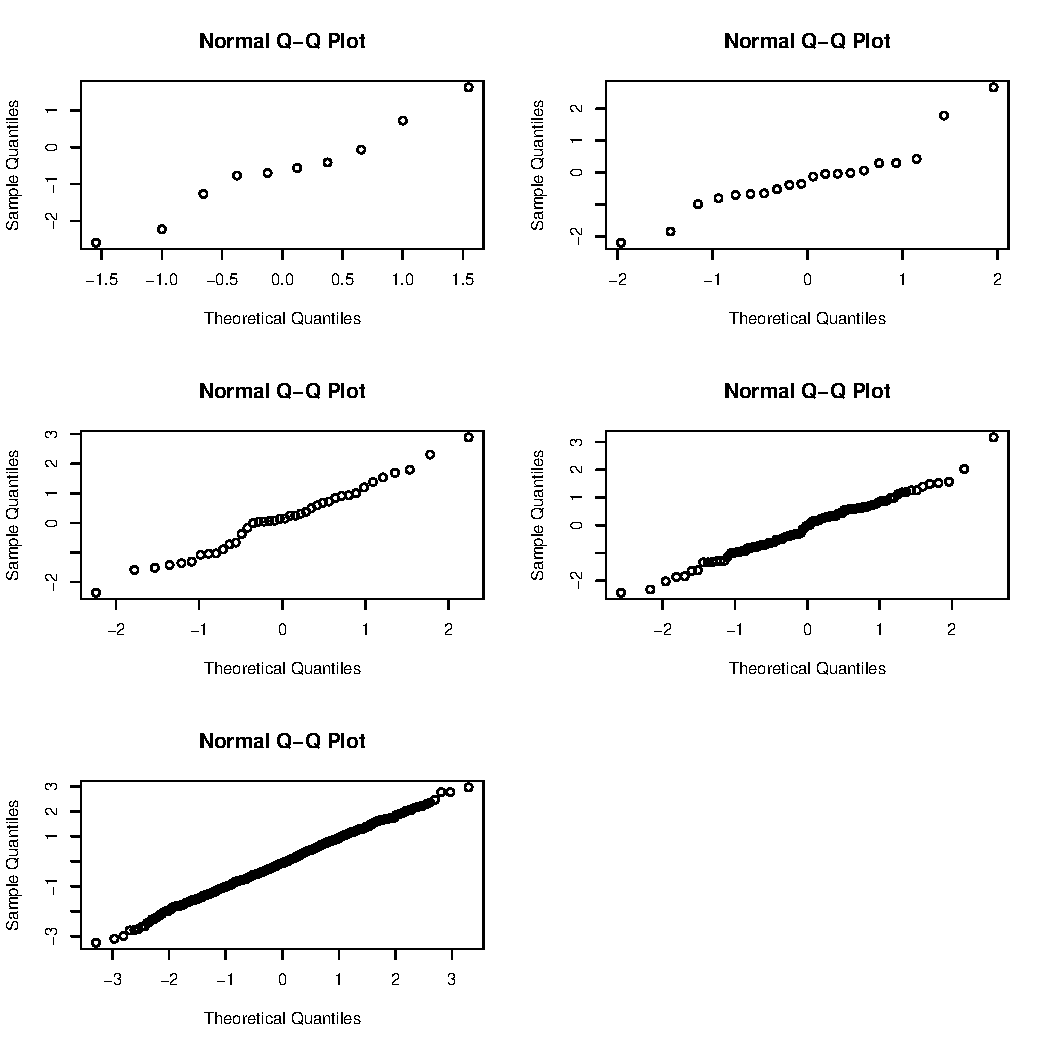
\includegraphics[width=\maxwidth]{figure/unnamed-chunk-2-3} 

\end{knitrout}

Rnorm with a size of 10 does not resemble anything like a line, Rnorm with a size of 20 does not resemble anything like a line, but shows some aspects of straightening out in the middle. Rnorm with a size of 40 is starting to straighten out in the middle. Rnorm with a size of 100 is straightening out in the middle a little more compared to size 40. Rnorm with a size of 1000 is almost completely straight in the middle, but not at the tail 

